\documentclass[conference]{IEEEtran}

\usepackage[T1]{fontenc}
\usepackage[utf8]{inputenc}
\usepackage[brazilian]{babel}
\usepackage{graphicx}
\usepackage{amsmath}
\usepackage{booktabs}
\usepackage{url}
\graphicspath{{./}}

\title{Introdução ao Processamento de Imagens: Aumento, Super-resolução e Realce}

\author{\IEEEauthorblockN{Luidgi Varela Carneiro}
\IEEEauthorblockA{Matrícula: 231011669\\
Universidade de Brasília}}

\begin{document}
\maketitle

\begin{abstract}
Este trabalho implementa três operações de aumento e combinação de imagens: repetição por fator dois (TAM2), interpolação por médias (TAMM) e inserção alternada de duas imagens (SUPERRES). Na Questão 1 foram utilizadas duas fotografias próprias do mesmo carrinho, obtidas de perspectivas ligeiramente diferentes. Na Questão 2 foram comparadas correção power-law, com quatro valores de gamma, e equalização de histograma nas imagens \,	exttt{car.png}, \,	exttt{crowd.png} e \,	exttt{university.png}. Os resultados mostram a preservação de blocos pela repetição, a suavização produzida pelas médias, a sensibilidade da SUPERRES ao desalinhamento e os efeitos distintos de gamma e da equalização sobre o contraste.
\end{abstract}

\section{Introdução}
O objetivo deste trabalho é estudar operações elementares de processamento digital de imagens e observar como diferentes estratégias alteram resolução aparente, continuidade espacial, brilho e contraste. A expansão por repetição atribui a cada amostra um bloco de pixels, preservando os valores originais, mas produzindo transições abruptas. A expansão por médias calcula valores intermediários a partir de amostras vizinhas, resultando em transições mais suaves.

Na correção power-law, cada intensidade normalizada $r$ é transformada por
\begin{equation}
    s = r^{\gamma}.
\end{equation}
Valores de $\gamma<1$ tendem a clarear a imagem, enquanto valores de $\gamma>1$ tendem a escurecê-la. A equalização de histograma utiliza a função de distribuição acumulada (CDF) para redistribuir as intensidades e ampliar o contraste global. Nas seções seguintes são descritos os métodos implementados, os resultados obtidos e as limitações observadas.

\section{Metodologia}
\subsection{Questão 1}
As duas fotografias próprias do carrinho foram preservadas em formato JPEG, RGB, com 864$\times$1536 pixels, sem redimensionamento. A função TAM2 foi implementada por chamadas sucessivas a uma operação de aumento por fator dois. Assim, foram executados os fatores 2 e 8 exigidos no enunciado.

Na TAMM, os pixels originais são colocados nas posições alternadas da imagem de saída. Quando há vizinhos disponíveis, os pixels horizontais, verticais e diagonais são calculados por médias aritméticas. Nas bordas, é usada a amostra disponível, reproduzindo o comportamento do exemplo do enunciado. A conversão para inteiros usa arredondamento para cima nos empates de meio valor, como no resultado esperado pelo exemplo.

A SUPERRES recebe as duas imagens com dimensões iguais. A primeira é escrita nas posições de linha e coluna ímpares, e a segunda nas posições pares, conforme a convenção de indexação do MATLAB. Não foi aplicado registro, alinhamento ou correção geométrica, pois isso alteraria o algoritmo solicitado. Matrizes artificiais também foram usadas para validar os valores e as posições das funções.

\subsection{Questão 2}
As três imagens fornecidas foram convertidas para tons de cinza e processadas com $\gamma\in\{0.4,0.7,1.4,2.2\}$. A transformação foi calculada sobre intensidades normalizadas e convertida novamente para o intervalo de 0 a 255. A equalização foi implementada a partir do histograma de 256 níveis e de sua CDF. Para a imagem \texttt{car.png}, foram salvos os histogramas e as CDFs antes e depois da operação.

\section{Resultados}
\subsection{Questão 1}
A Figura~\ref{fig:q1} reúne as fotografias e os principais resultados. TAM2 fator 2, TAMM e SUPERRES produziram imagens de 1728$\times$3072 pixels; TAM2 fator 8 produziu 6912$\times$12288 pixels. A TAM2 preserva os valores de cada amostra e repete blocos, sendo simples e previsível, mas sem suavização. A TAMM apresenta aparência mais contínua, pois interpola as posições intermediárias por médias.

Na SUPERRES, a diferença entre as perspectivas causa duplicações, deslocamentos e contornos inconsistentes em regiões do carrinho. Além disso, como a função posiciona somente as duas grades especificadas, a imagem resultante é esparsa nas demais posições. Esses artefatos não foram escondidos por alinhamento posterior: eles documentam a limitação de combinar aquisições que não são perfeitamente coincidentes.

\begin{figure*}[t]
\centering
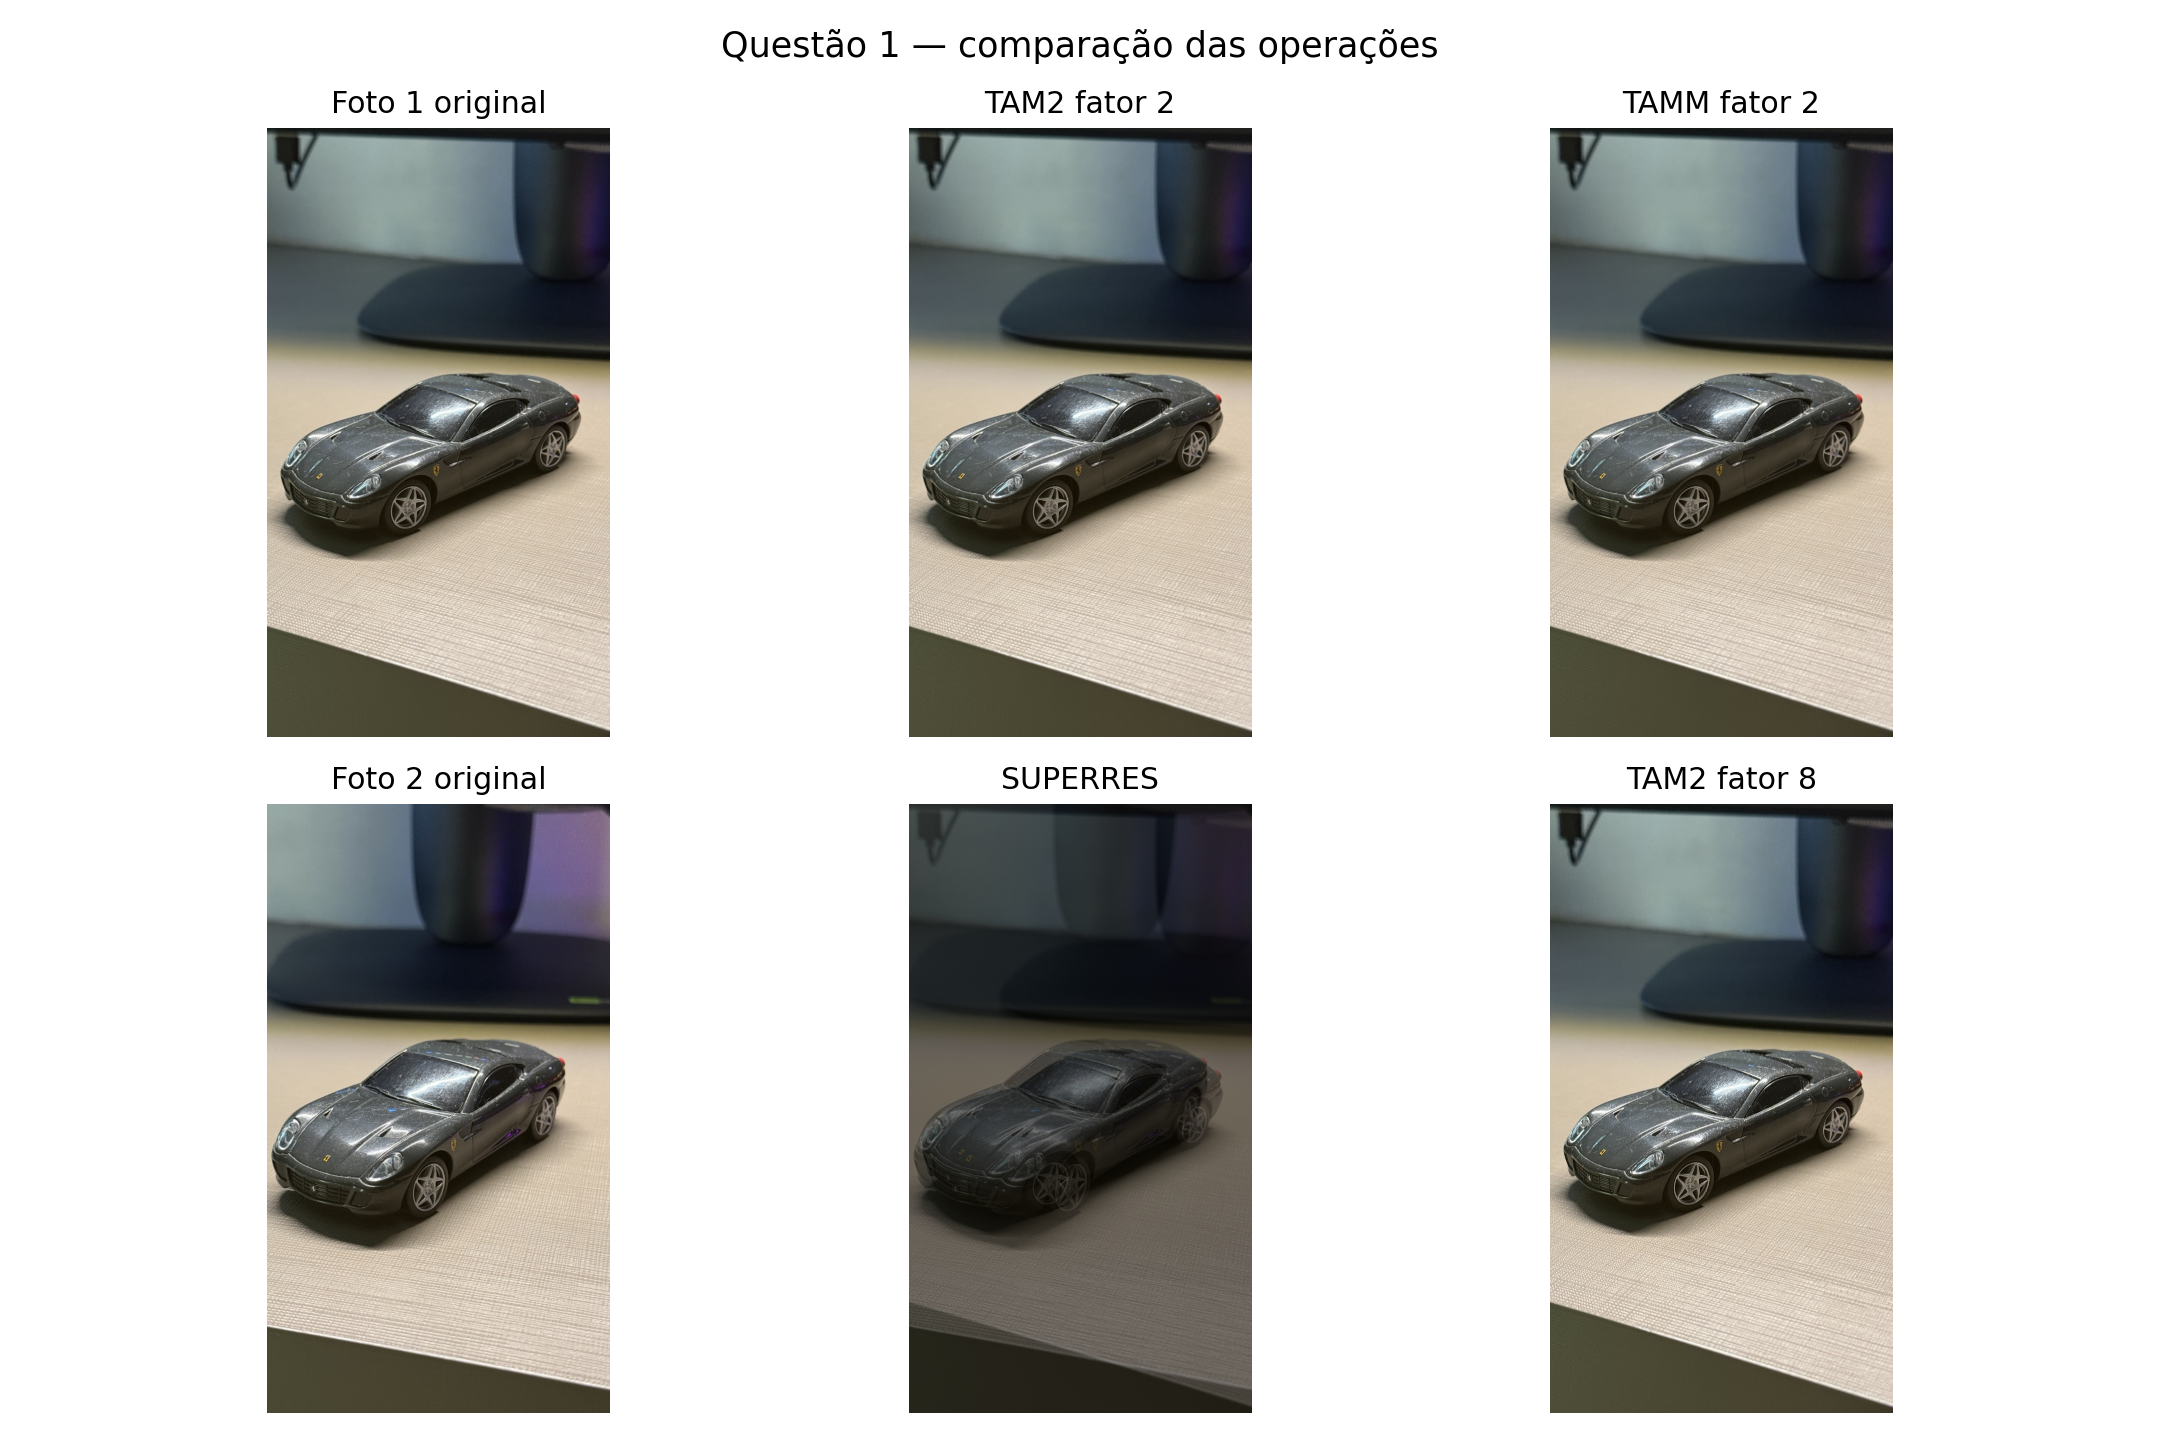
\includegraphics[width=0.94\textwidth]{q1_comparacao.png}
\caption{Fotografias próprias e resultados de TAM2, TAMM e SUPERRES.}
\label{fig:q1}
\end{figure*}

\subsection{Questão 2}
A Figura~\ref{fig:q2} mostra uma comparação compacta dos métodos. Para as alternativas testadas, foram destacados como melhores compromissos de visibilidade $\gamma=0.7$ para \texttt{car}, $\gamma=0.4$ para \texttt{crowd} e $\gamma=0.4$ para \texttt{university}. Os valores menores que um revelaram detalhes em regiões escuras, enquanto os valores maiores que um escureceram as cenas e reduziram a informação visual em áreas já pouco iluminadas.

\begin{figure*}[t]
\centering
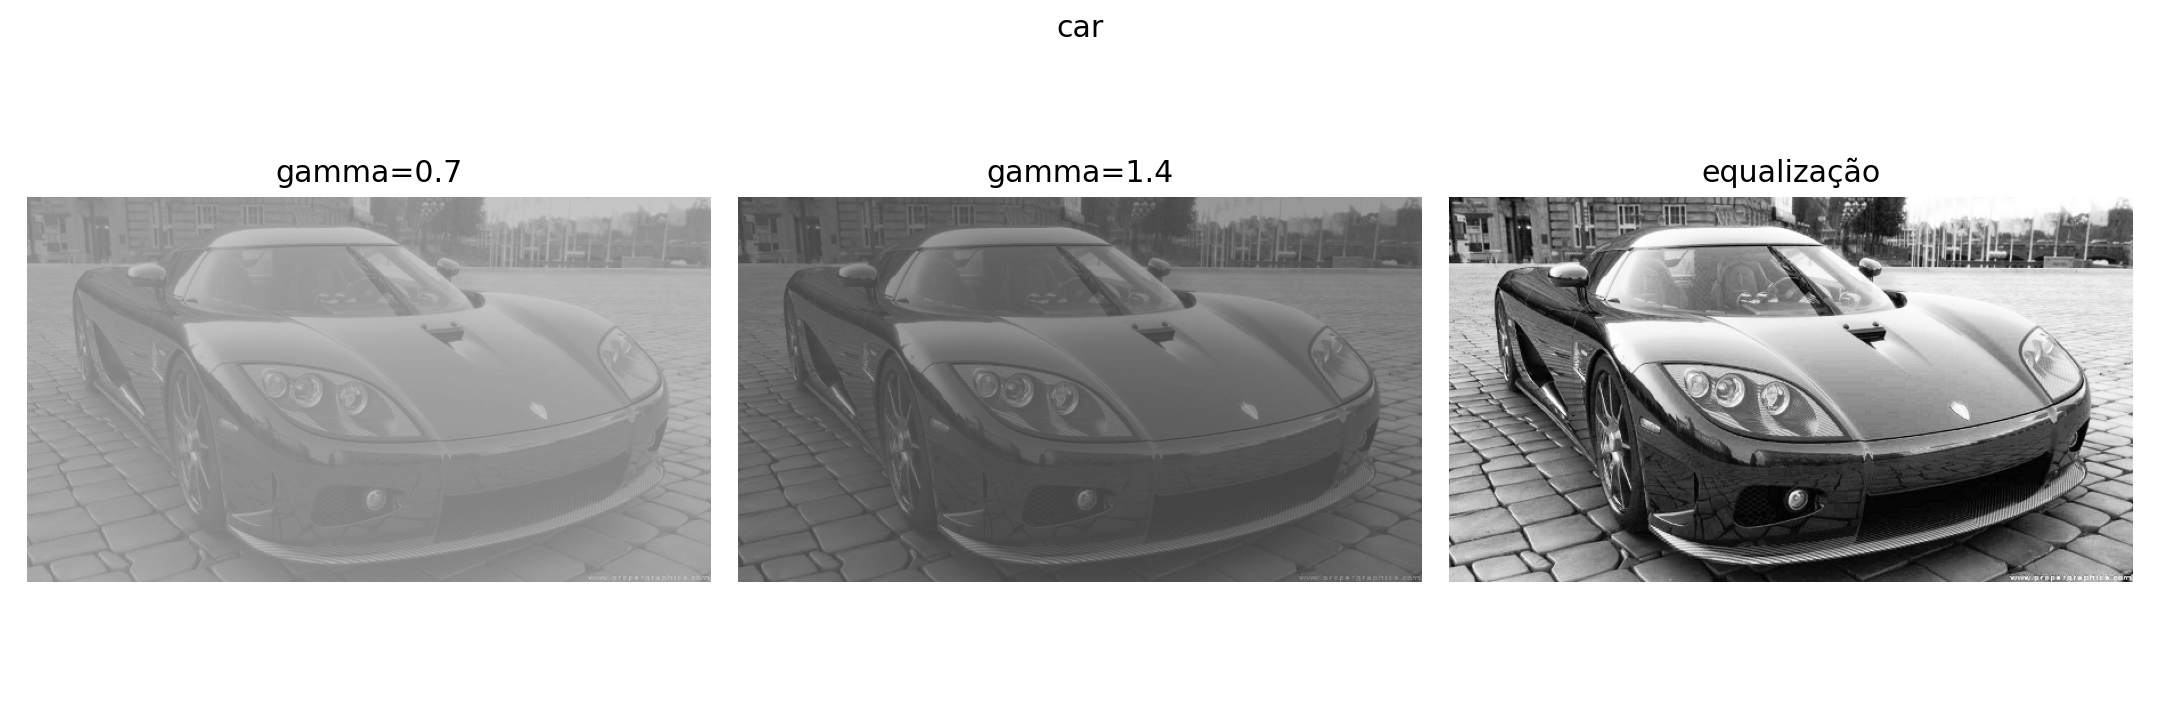
\includegraphics[width=0.32\textwidth]{car_comparacao.png}\hfill
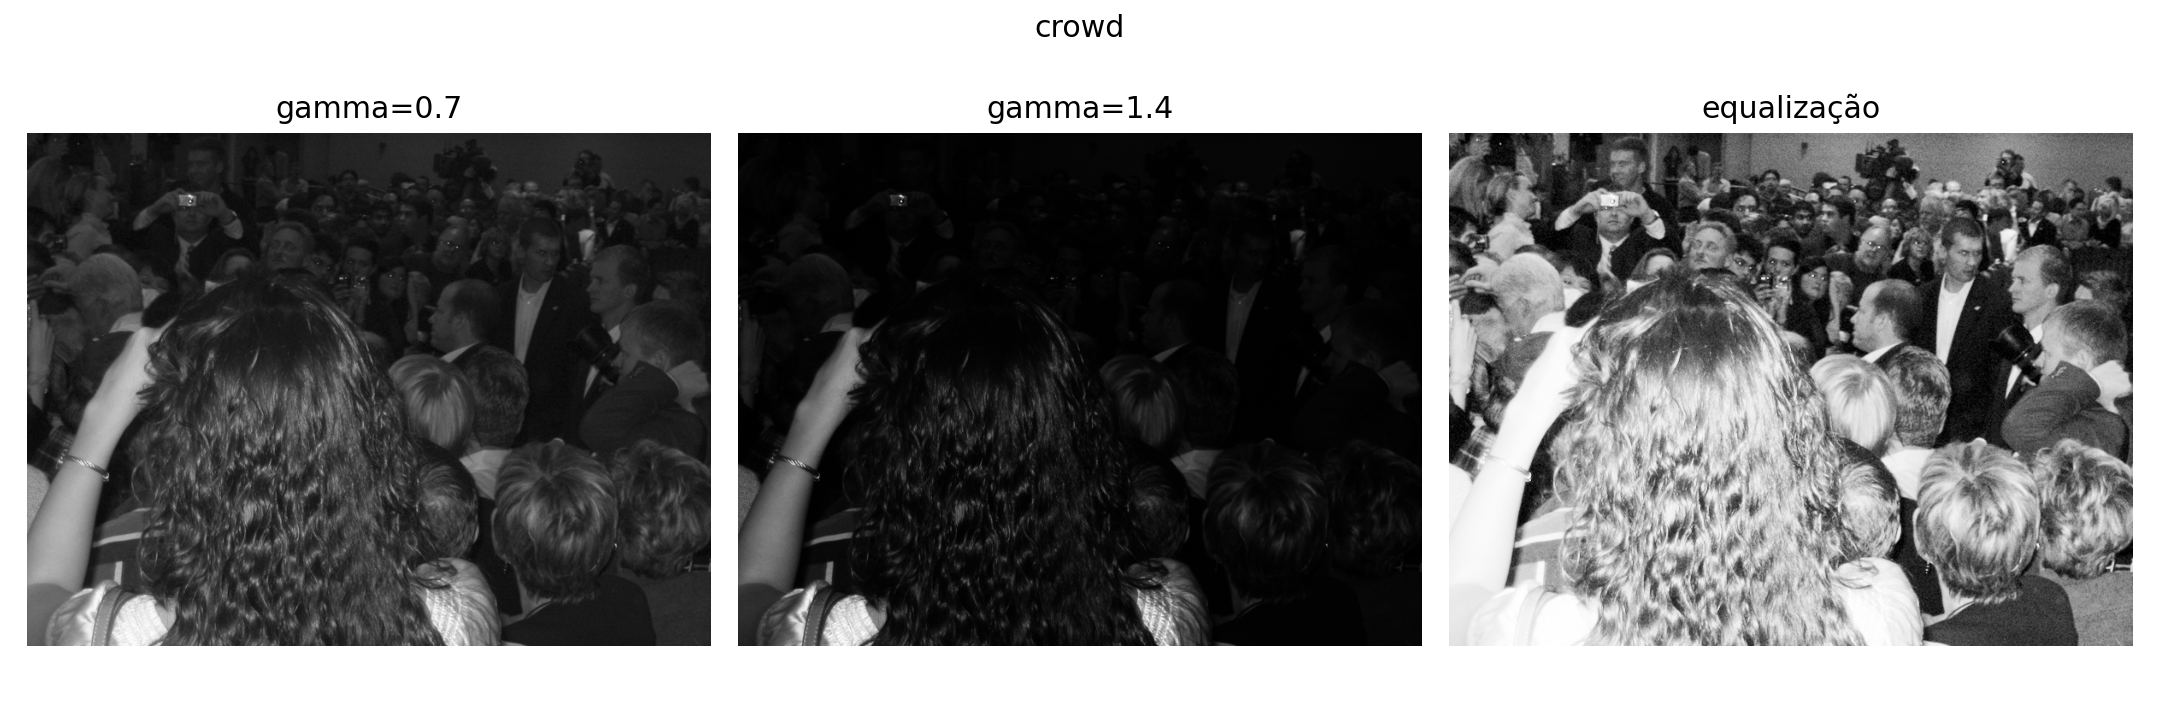
\includegraphics[width=0.32\textwidth]{crowd_comparacao.png}\hfill
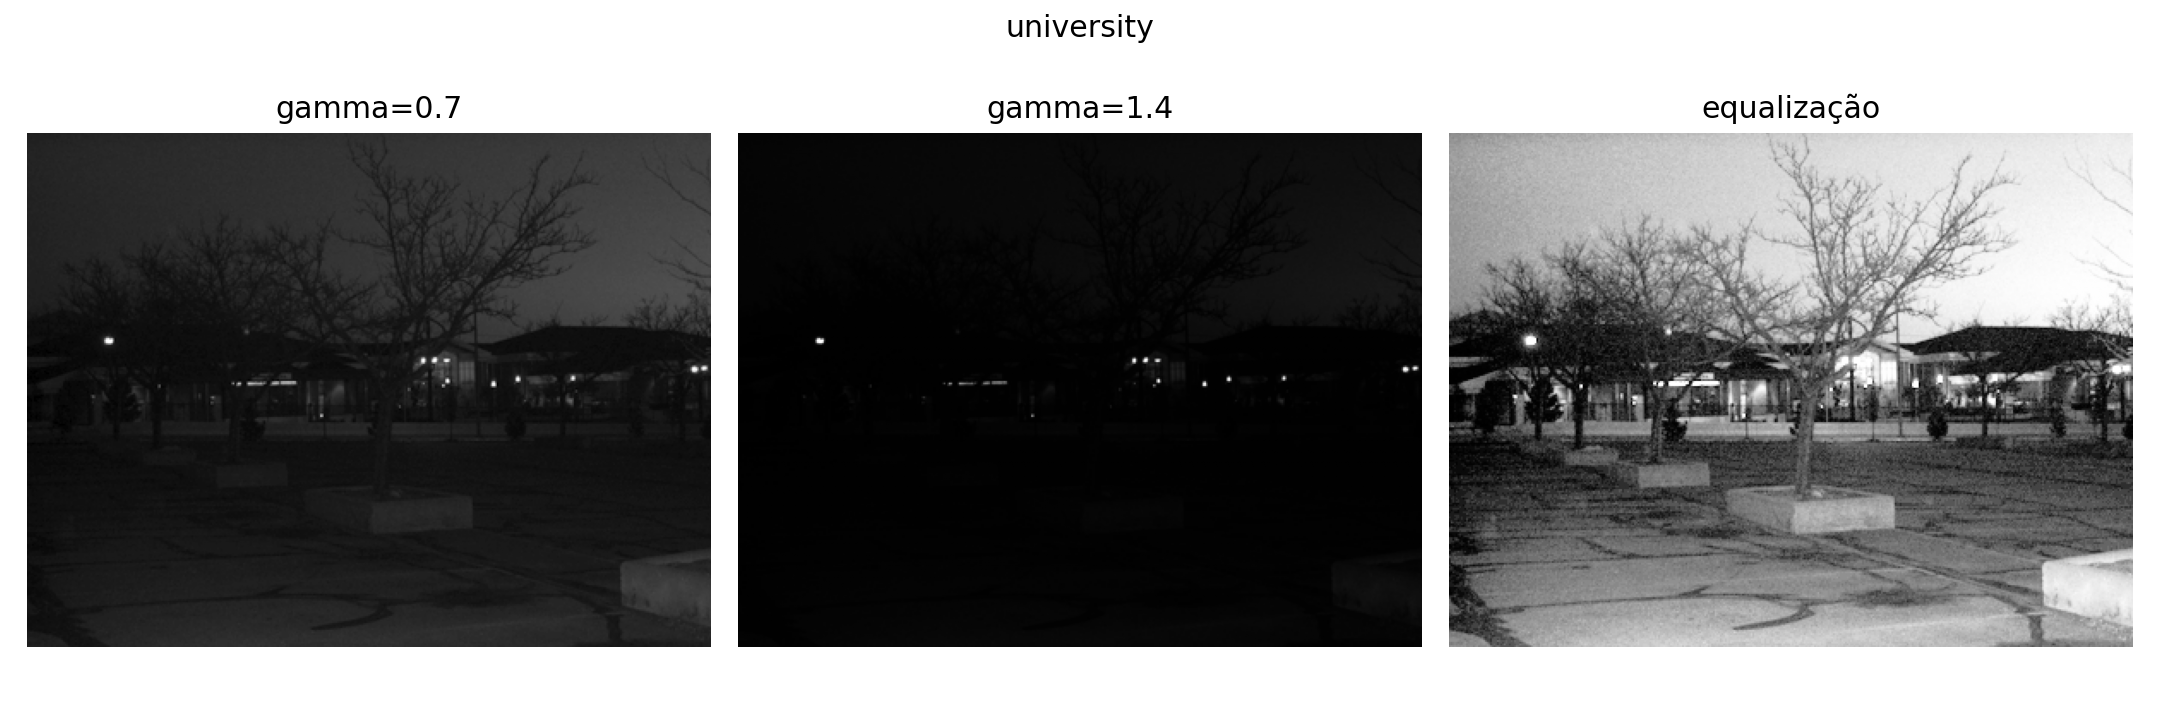
\includegraphics[width=0.32\textwidth]{university_comparacao.png}
\caption{Comparações entre correção gamma e equalização para as três imagens.}
\label{fig:q2}
\end{figure*}

Na imagem \texttt{car}, a equalização produz contraste mais forte que as duas alternativas gamma exibidas. Na imagem \texttt{crowd}, ela revela detalhes em diferentes regiões da cena, embora também intensifique diferenças locais. Na imagem \texttt{university}, originalmente escura, a equalização amplia a visibilidade da praça e das árvores. Assim, gamma é mais controlável para ajustar brilho, enquanto a equalização é mais apropriada quando se busca uma redistribuição global do contraste.

\clearpage
\begin{center}
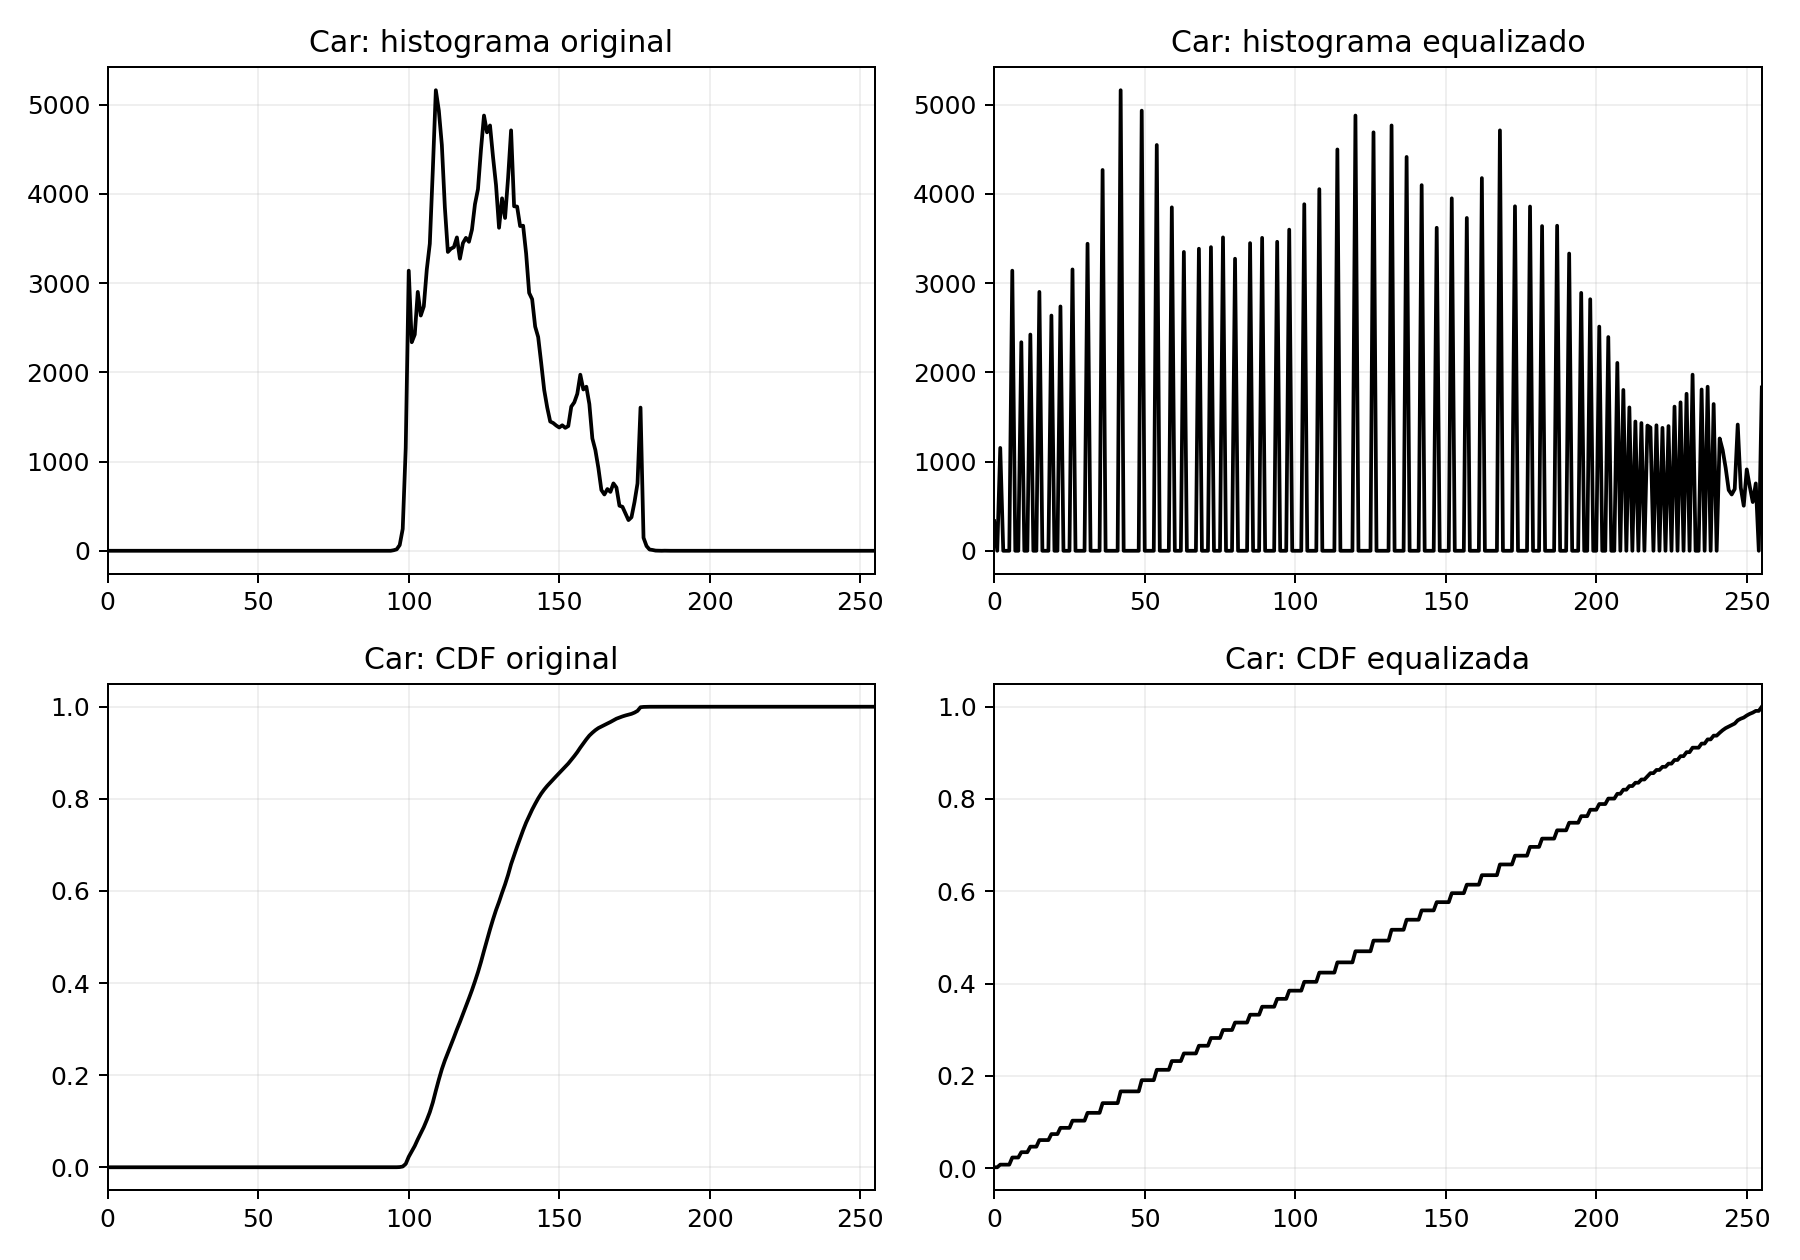
\includegraphics[width=0.96\columnwidth]{car_histogramas_cdfs.png}\\[-1mm]
\footnotesize\textbf{Fig. 3.} Histogramas e CDF da imagem \texttt{car} antes e depois da equalização.
\end{center}

Como mostra a Fig. 3, a equalização desloca a distribuição dos níveis e espalha a CDF pelo intervalo de intensidades. As médias e os desvios-padrão dos quatro valores de gamma para cada imagem foram registrados em \texttt{metricas\_gamma.csv}; eles confirmam numericamente a tendência visual de clareamento para $\gamma<1$ e escurecimento para $\gamma>1$.

\section{Conclusões}
As validações numéricas confirmaram a repetição de linhas e colunas na TAM2, os valores médios da TAMM e o posicionamento alternado das duas imagens na SUPERRES. Nas fotografias reais, a TAM2 foi a operação mais simples e preservou blocos, a TAMM produziu uma aparência mais contínua e a SUPERRES evidenciou a sensibilidade a diferenças de perspectiva e a posições não preenchidas.

Na Questão 2, a correção gamma permitiu controlar diretamente o brilho e foi especialmente útil para revelar regiões escuras com valores menores que um. A equalização modificou mais intensamente o contraste global e apresentou ganhos visuais nas três imagens, acompanhados de alterações correspondentes nos histogramas e CDFs. Todos os resultados discutidos foram gerados pelo código do projeto e estão organizados nas pastas de resultados.

\end{document}
